\documentclass[11pt,a4paper]{report}
\usepackage[textwidth=37em,vmargin=30mm]{geometry}
\usepackage{calc,xunicode,amsmath,amssymb,paralist,enumitem,tabu,booktabs,datetime2,xeCJK,xeCJKfntef,listings}
\usepackage{tocloft,fancyhdr,tcolorbox,xcolor,graphicx,eso-pic,xltxtra,xelatexemoji}

\newcommand{\envyear}[0]{2025}
\newcommand{\envdatestr}[0]{2025-01-27}
\newcommand{\envfinaldir}[0]{webdb/2025/20250127/final}

\usepackage[hidelinks]{hyperref}
\hypersetup{
    colorlinks=false,
    pdfpagemode=FullScreen,
    pdftitle={Web Digest - \envdatestr}
}

\setlength{\cftbeforechapskip}{10pt}
\renewcommand{\cftchapfont}{\rmfamily\bfseries\large\raggedright}
\setlength{\cftbeforesecskip}{2pt}
\renewcommand{\cftsecfont}{\sffamily\small\raggedright}

\setdefaultleftmargin{2em}{2em}{1em}{1em}{1em}{1em}

\usepackage{xeCJK,xeCJKfntef}
\xeCJKsetup{PunctStyle=plain,RubberPunctSkip=false,CJKglue=\strut\hskip 0pt plus 0.1em minus 0.05em,CJKecglue=\strut\hskip 0.22em plus 0.2em}
\XeTeXlinebreaklocale "zh"
\XeTeXlinebreakskip = 0pt


\setmainfont{Brygada 1918}
\setromanfont{Brygada 1918}
\setsansfont{IBM Plex Sans}
\setmonofont{JetBrains Mono NL}
\setCJKmainfont{Noto Serif CJK SC}
\setCJKromanfont{Noto Serif CJK SC}
\setCJKsansfont{Noto Sans CJK SC}
\setCJKmonofont{Noto Sans CJK SC}

\setlength{\parindent}{0pt}
\setlength{\parskip}{8pt}
\linespread{1.15}

\lstset{
	basicstyle=\ttfamily\footnotesize,
	numbersep=5pt,
	backgroundcolor=\color{black!5},
	showspaces=false,
	showstringspaces=false,
	showtabs=false,
	tabsize=2,
	captionpos=b,
	breaklines=true,
	breakatwhitespace=true,
	breakautoindent=true,
	linewidth=\textwidth
}






\newcommand{\coverpic}[2]{
    % argv: itemurl, authorname
    Cover photo by #2~~(\href{#1}{#1})
}
\newcommand{\makeheader}[0]{
    \begin{titlepage}
        % \newgeometry{hmargin=15mm,tmargin=21mm,bmargin=12mm}
        \begin{center}
            
            \rmfamily\scshape
            \fontspec{BaskervilleF}
            \fontspec{Old Standard}
            \fontsize{59pt}{70pt}\selectfont
            WEB\hfill DIGEST
            
            \vfill
            % \vskip 30pt
            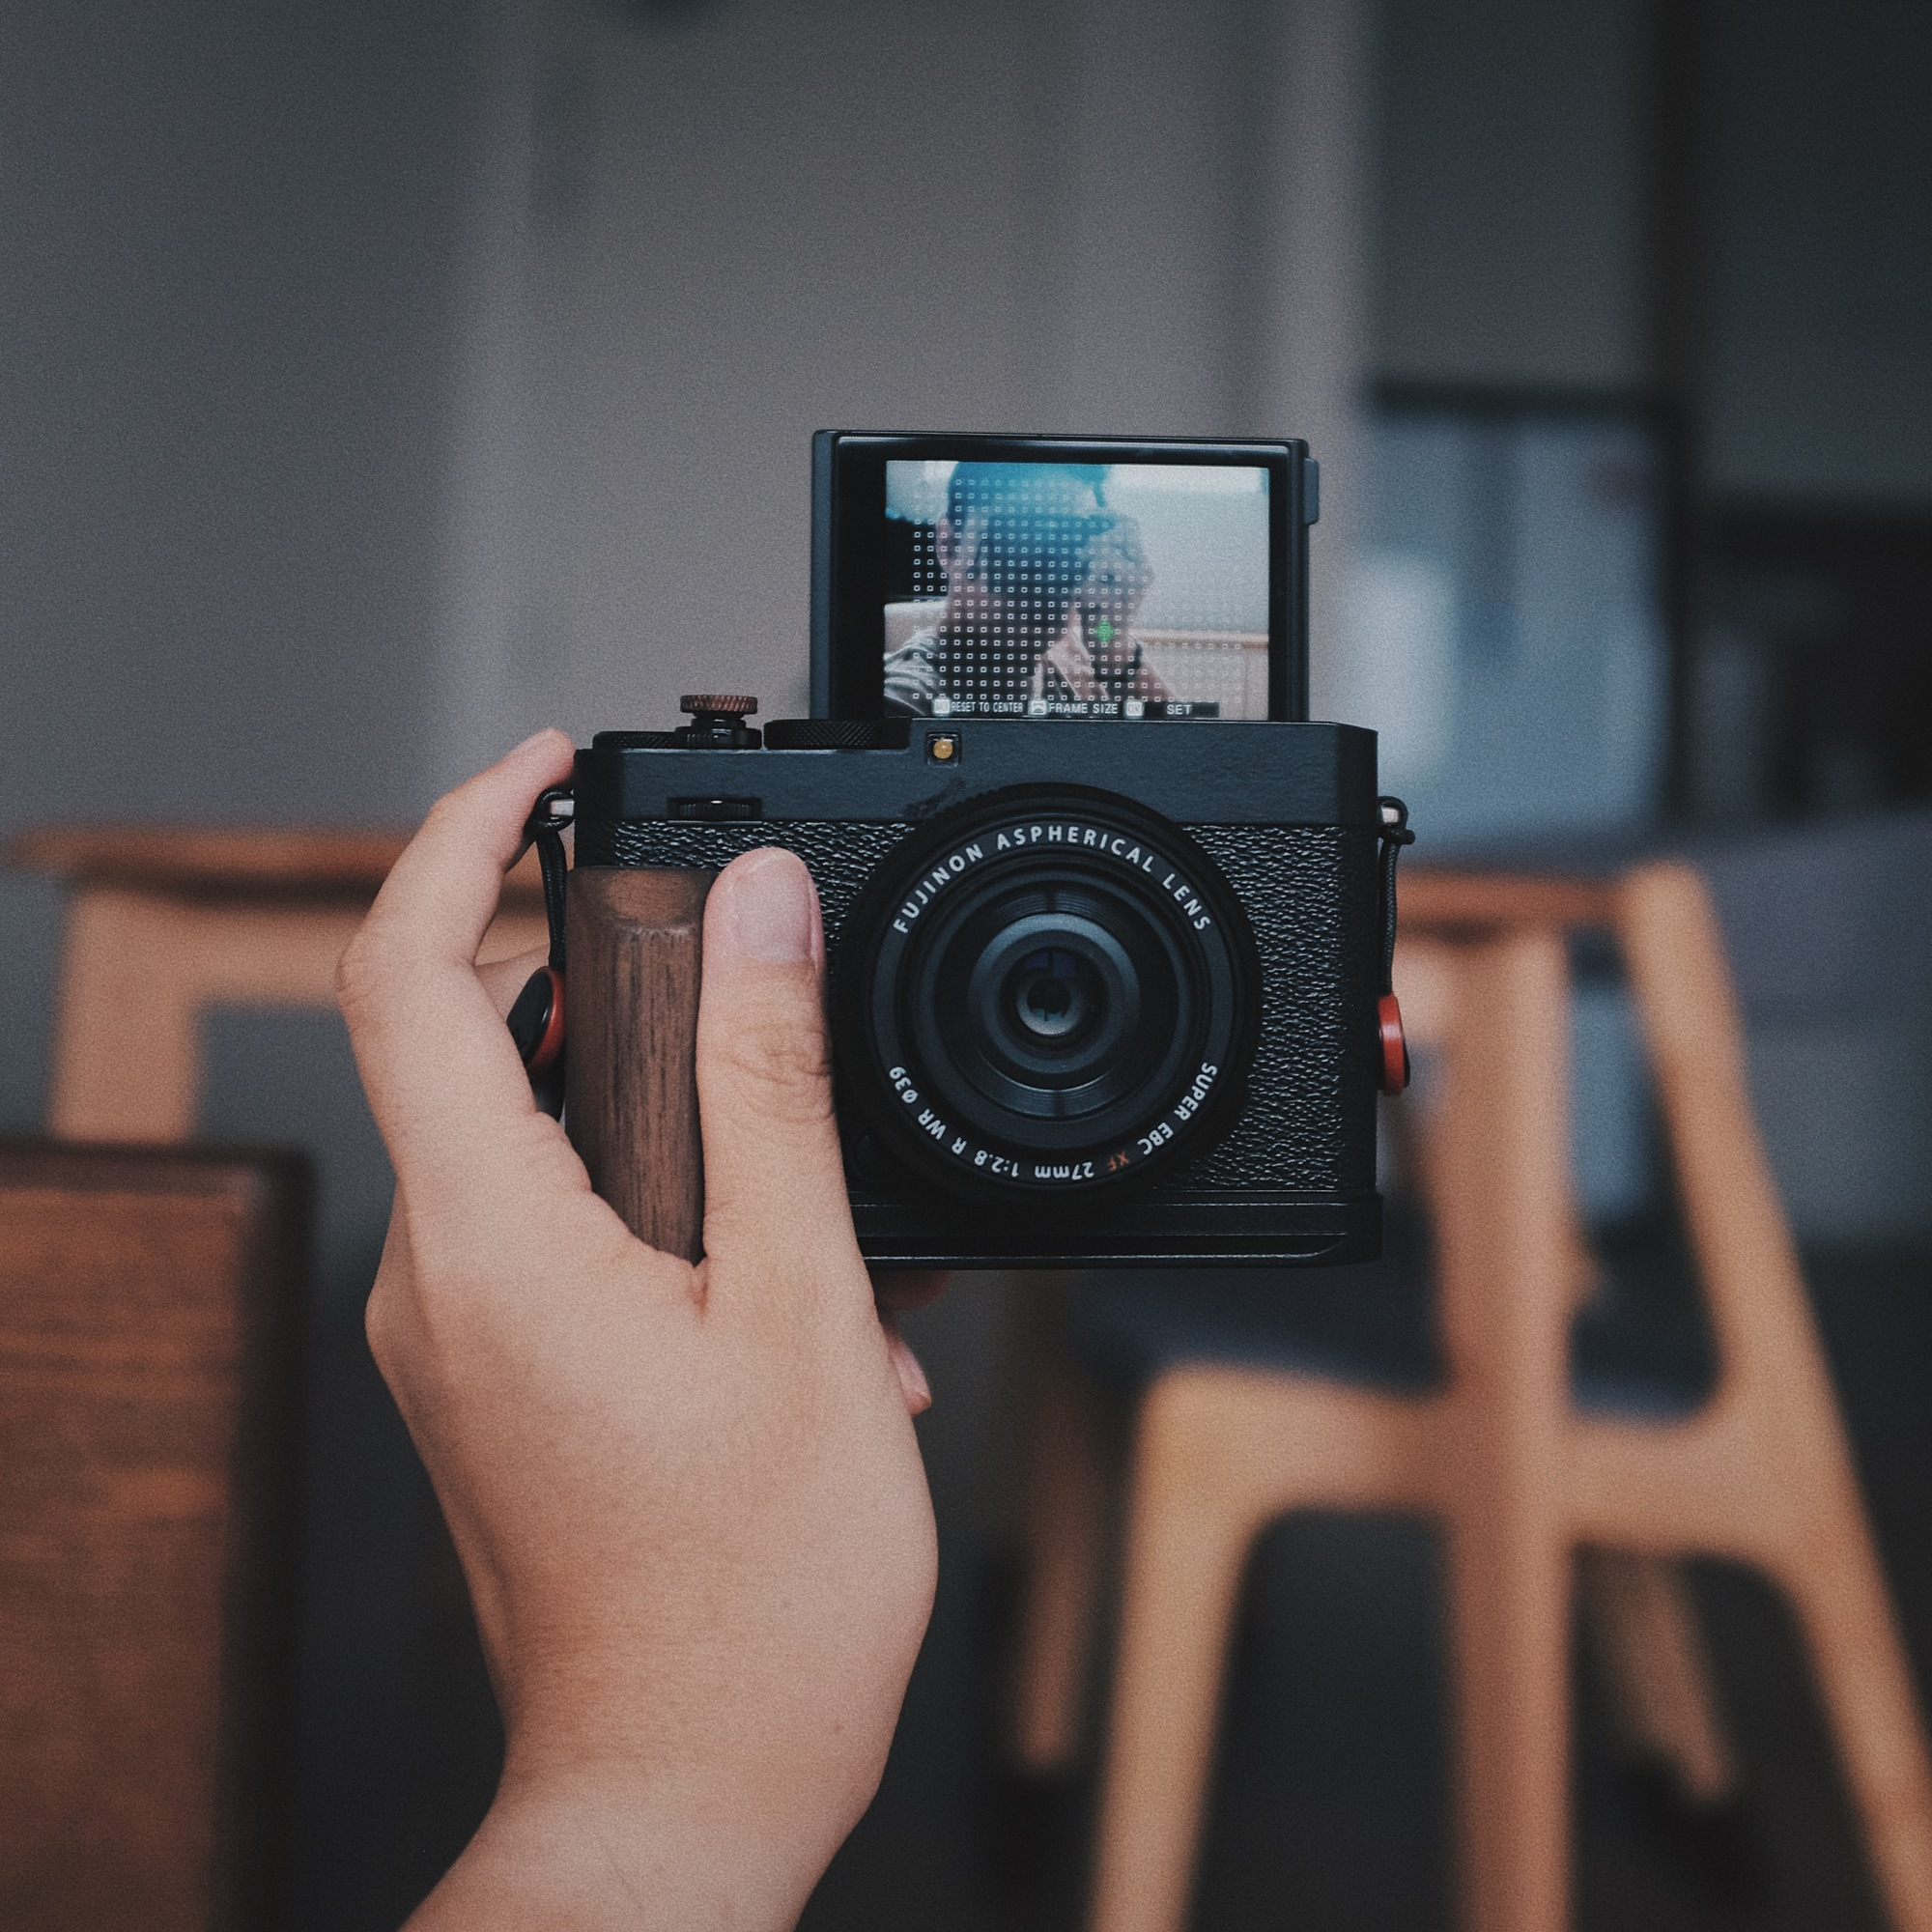
\includegraphics[width=\linewidth]{\envfinaldir/coverpic-prod.jpg}\par
            % \vskip 30pt
            \vfill

            \normalsize\rmfamily\scshape
            \copyright{} The Web Digest Project \hfill\large \envdatestr
        \end{center}
    \end{titlepage}
    % \restoregeometry
}
\newcommand{\simplehref}[1]{%
    \textcolor{blue!80!green}{\href{#1}{#1}}%
}
\renewcommand{\contentsname}{\center\Huge\sffamily\bfseries Contents\par\vskip 20pt}
\newcounter{ipartcounter}
\setcounter{ipartcounter}{0}
\newcommand{\ipart}[1]{
    % \vskip 20pt
    \clearpage
    \stepcounter{ipartcounter}
    \phantomsection
    \addcontentsline{toc}{chapter}{#1}
    % \begin{center}
    %     \Huge
    %     \sffamily\bfseries
    %     #1
    % \end{center}
    % \vskip 20pt plus 7pt
}
\newcounter{ichaptercounter}
\setcounter{ichaptercounter}{0}
\newcommand{\ichapter}[1]{
    % \vskip 20pt
    \clearpage
    \stepcounter{ichaptercounter}
    \phantomsection
    \addcontentsline{toc}{section}{\numberline{\arabic{ichaptercounter}}#1}
    \begin{center}
        \Huge
        \sffamily\bfseries
        #1
    \end{center}
    \vskip 20pt plus 7pt
}
\newcommand{\entrytitlefont}[1]{\subsection*{\raggedright\Large\sffamily\bfseries#1}}
\newcommand{\entryitemGeneric}[2]{
    % argv: title, url
    \parbox{\linewidth}{
        \entrytitlefont{#1}\par\vskip 5pt
        \footnotesize\ttfamily\mdseries
        \simplehref{#2}
    }\vskip 11pt plus 11pt minus 1pt
}
\newcommand{\entryitemGithub}[3]{
    % argv: title, url, desc
    \parbox{\linewidth}{
        \entrytitlefont{#1}\par\vskip 5pt
        \footnotesize\ttfamily\mdseries
        \simplehref{#2}\par\vskip 5pt
        \small\rmfamily\mdseries#3
    }\vskip 11pt plus 11pt minus 1pt
}
\newcommand{\entryitemAp}[3]{
    % argv: title, url, desc
    \parbox{\linewidth}{
        \entrytitlefont{#1}\par\vskip 5pt
        \footnotesize\ttfamily\mdseries
        \simplehref{#2}\par\vskip 5pt
        \small\rmfamily\mdseries#3
    }\vskip 11pt plus 11pt minus 1pt
}
\newcommand{\entryitemHackernews}[3]{
    % argv: title, hnurl, rawurl
    % \parbox{\linewidth}{
    %     \entrytitlefont{#1}\par\vskip 5pt
    %     \footnotesize\ttfamily\mdseries
    %     \simplehref{#3}\par
    %     \textcolor{black!50}{\href{#2}{#2}}
    % }\vskip 11pt plus 11pt minus 1pt
    \begin{minipage}{\linewidth}
            \entrytitlefont{#1}\par\vskip 5pt
            \footnotesize\ttfamily\mdseries
            \simplehref{#3}\par
            \textcolor{black!50}{\href{#2}{#2}}
    \end{minipage}\par\vskip 11pt plus 11pt minus 1pt
}







\begin{document}

\makeheader

\tableofcontents\clearpage




\ipart{Developers}
\ichapter{Hacker News}
\entryitemTwoLinks{Mark Zuckerberg: This Man Is a Coward}{https://news.ycombinator.com/item?id=42834911}{https://www.theindex.media/this-man-is-a-coward/}

\entryitemTwoLinks{Show HN: DeepSeek My User Agent}{https://news.ycombinator.com/item?id=42834648}{https://www.jasonthorsness.com/20}

\entryitemTwoLinks{Brazil bans Sam Altman's tech firm Tools for Humanity from paying for iris scans}{https://news.ycombinator.com/item?id=42834432}{https://economictimes.indiatimes.com/tech/technology/brazil-bans-sam-altmans-tech-firm-tools-for-humanity-from-paying-for-iris-scans/articleshow/117540826.cms?from=mdr}

\entryitemTwoLinks{Another undersea cable damaged in Baltic Sea}{https://news.ycombinator.com/item?id=42833491}{https://www.france24.com/en/europe/20250126-another-undersea-cable-damaged-in-baltic-sea-latvia-dispatches-warship}

\entryitemTwoLinks{Former tech CEO suing to get the record of his arrest removed from the internet}{https://news.ycombinator.com/item?id=42833193}{https://sf.gazetteer.co/a-former-tech-ceo-is-on-a-crusade-to-get-the-record-of-his-arrest-removed-from-the-internet}

\entryitemTwoLinks{No Bitcoin ETFs at Vanguard (2024)}{https://news.ycombinator.com/item?id=42832026}{https://corporate.vanguard.com/content/corporatesite/us/en/corp/articles/no-bitcoin-etfs-at-vanguard-heres-why.html}

\entryitemTwoLinks{Qwen2.5-1M: Deploy your own Qwen with context length up to 1M tokens}{https://news.ycombinator.com/item?id=42831769}{https://qwenlm.github.io/blog/qwen2.5-1m/}

\entryitemTwoLinks{Hard numbers in the Wayland vs. X11 input latency discussion}{https://news.ycombinator.com/item?id=42831509}{https://mort.coffee/home/wayland-input-latency/}

\entryitemTwoLinks{The Microsoft 365 Copilot launch was a disaster}{https://news.ycombinator.com/item?id=42831281}{https://www.zdnet.com/home-and-office/work-life/the-microsoft-365-copilot-launch-was-a-total-disaster/}

\entryitemTwoLinks{It's not a crime if we do it with an app}{https://news.ycombinator.com/item?id=42830646}{https://pluralistic.net/2025/01/25/potatotrac/\#carbo-loading}

\entryitemTwoLinks{When AI promises speed but delivers debugging hell}{https://news.ycombinator.com/item?id=42829466}{https://nsavage.substack.com/p/when-ai-promises-speed-but-delivers}

\entryitemTwoLinks{The protester's guide to smartphone security}{https://news.ycombinator.com/item?id=42829317}{https://www.privacyguides.org/articles/2025/01/23/activists-guide-securing-your-smartphone/}

\entryitemTwoLinks{Paxo: A DIY Phone}{https://news.ycombinator.com/item?id=42829279}{https://paxo.fr/}

\entryitemTwoLinks{YC Graveyard: 821 inactive Y Combinator startups}{https://news.ycombinator.com/item?id=42828198}{https://ycgraveyard.iamwillwang.com/}

\entryitemTwoLinks{Ask HN: Anyone else find LLM related posts causing them to lose interest in HN}{https://news.ycombinator.com/item?id=42827723}{https://news.ycombinator.com/item?id=42827723}

\entryitemTwoLinks{Explainer: What's r1 and everything else?}{https://news.ycombinator.com/item?id=42827601}{https://timkellogg.me/blog/2025/01/25/r1}

\entryitemTwoLinks{AI slop, suspicion, and writing back}{https://news.ycombinator.com/item?id=42827532}{https://benjamincongdon.me/blog/2025/01/25/AI-Slop-Suspicion-and-Writing-Back/}

\entryitemTwoLinks{Emerging reasoning with reinforcement learning}{https://news.ycombinator.com/item?id=42827399}{https://hkust-nlp.notion.site/simplerl-reason}

\entryitemTwoLinks{The Simplicity of Prolog}{https://news.ycombinator.com/item?id=42827335}{https://bitsandtheorems.com/the-simplicity-of-prolog/}

\entryitemTwoLinks{The South Vietnamese pilot who landed a Cessna on a carrier to save his family (2019)}{https://news.ycombinator.com/item?id=42826536}{https://www.historynet.com/maj-buang-lys-daring-feat-to-save-his-family/}\ichapter{Phoronix}
\entryitemGeneric{\hskip 0pt{}ARCTIC Freezer 4U-M Cooler For Ampere Altra 4U Servers/Workstations}{https://www.phoronix.com/review/arctic-freezer-4u-m-ampere}

\entryitemGeneric{\hskip 0pt{}AMD Squeezes In More RDNA4 Changes For Linux 6.14 - Enables Cleaner Shader On GFX12}{https://www.phoronix.com/news/AMDGPU-More-GFX12-Linux-6.14}

\entryitemGeneric{\hskip 0pt{}Linux Patches Allow Sharing PTEs Between Processes - Can Mean Significant RAM Savings}{https://www.phoronix.com/news/Linux-Sharing-PTEs-Processes}

\entryitemGeneric{\hskip 0pt{}Mesa 25.0 Gets A New Vulkan Layer For Limiting The Amount Of Reported vRAM}{https://www.phoronix.com/news/Mesa-Vulkan-vRAM-Report-Limit}

\entryitemGeneric{\hskip 0pt{}New Sound Hardware Supported By The Linux 6.14 Kernel}{https://www.phoronix.com/news/Linux-6.14-New-Sound-Hardware}

\entryitemGeneric{\hskip 0pt{}Linux 6.14 Adds ROCEv2 Support For The Alibaba Cloud}{https://www.phoronix.com/news/Linux-6.14-RDMA}

\entryitemGeneric{\hskip 0pt{}Shotcut 25.01 Open-Source Video Editor Brings New Features}{https://www.phoronix.com/news/Shotcut-25.01-Released}

\entryitemGeneric{\hskip 0pt{}Intel Media Driver 2024Q4 Released With Battlemage Video Encode}{https://www.phoronix.com/news/Intel-Media-Driver-2024Q4}

\entryitemGeneric{\hskip 0pt{}ISD: A New Interactive Way For systemd Management}{https://www.phoronix.com/news/ISD-Interactive-Systemd}


\ipart{Developers~~~~(zh-Hans)}
\ichapter{Solidot}
\entryitemGeneric{\hskip 0pt{}GLP-1RA 的益处和风险}{https://www.solidot.org/story?sid=80431}

\entryitemGeneric{\hskip 0pt{}研究人员发现中欧电网用非加密无线信号控制}{https://www.solidot.org/story?sid=80430}

\entryitemGeneric{\hskip 0pt{}甲骨文等正在谈判接手 TikTok 美国业务}{https://www.solidot.org/story?sid=80428}

\entryitemGeneric{\hskip 0pt{}小鼠研究发现微塑料会堵塞大脑血液流动}{https://www.solidot.org/story?sid=80427}

\entryitemGeneric{\hskip 0pt{}ADHD 患者有更短的预期寿命}{https://www.solidot.org/story?sid=80426}

\entryitemGeneric{\hskip 0pt{}研究称电动汽车的寿命与燃油汽车相差无几}{https://www.solidot.org/story?sid=80425}

\entryitemGeneric{\hskip 0pt{}大英博物馆遭前 IT 雇员攻击而部分关闭}{https://www.solidot.org/story?sid=80424}

\entryitemGeneric{\hskip 0pt{}巴基斯坦议会通过法案全面控制社交媒体}{https://www.solidot.org/story?sid=80423}

\entryitemGeneric{\hskip 0pt{}AI 犯的错误和人类不同}{https://www.solidot.org/story?sid=80422}

\entryitemGeneric{\hskip 0pt{}数百超级富豪呼吁对其征收更高的税}{https://www.solidot.org/story?sid=80421}

\entryitemGeneric{\hskip 0pt{}Linux 6.14 加入对微软 Copilot 按键的支持}{https://www.solidot.org/story?sid=80420}

\entryitemGeneric{\hskip 0pt{}秘密后门使用``魔法封包''感染企业 VPN}{https://www.solidot.org/story?sid=80419}

\entryitemGeneric{\hskip 0pt{}调查显示八成游戏开发商开发 PC 游戏}{https://www.solidot.org/story?sid=80418}

\entryitemGeneric{\hskip 0pt{}《自然》调查显示七成回应者使用 Bluesky}{https://www.solidot.org/story?sid=80417}

\entryitemGeneric{\hskip 0pt{}乔治 R.R.马丁合作发表了一篇物理学论文}{https://www.solidot.org/story?sid=80416}

\entryitemGeneric{\hskip 0pt{}Google 移动搜索移除网址面包屑导航}{https://www.solidot.org/story?sid=80415}

\entryitemGeneric{\hskip 0pt{}癌细胞利用有缺陷的线粒体毒害攻击免疫细胞}{https://www.solidot.org/story?sid=80414}

\entryitemGeneric{\hskip 0pt{}日本市场中国平板电视首次超过五成}{https://www.solidot.org/story?sid=80413}

\entryitemGeneric{\hskip 0pt{}智人离开非洲后血型可能发生适应性遗传变化}{https://www.solidot.org/story?sid=80412}

\entryitemGeneric{\hskip 0pt{}三菱不打算参与本田日产的合并}{https://www.solidot.org/story?sid=80411}\ichapter{V2EX}
\entryitemGeneric{\hskip 0pt{}[macOS] 终于解决了困扰大半年(不止)的 Caps 切换中英文不顺手的问题了}{https://www.v2ex.com/t/1108027}

\entryitemGeneric{\hskip 0pt{}[分享创造] 啥?中产不适合移民?聊聊我为什么适合移民}{https://www.v2ex.com/t/1108026}

\entryitemGeneric{\hskip 0pt{}[问与答] 群晖上跑 qbittorrent docker, 一直显示 "下载元数据", 但是用种子文件直接下载就可以}{https://www.v2ex.com/t/1108025}

\entryitemGeneric{\hskip 0pt{}[游戏开发] 现在手机游戏冷启动一个比一个慢,是否是为了延长轻度玩家游戏时间有意为之的行为?}{https://www.v2ex.com/t/1108024}

\entryitemGeneric{\hskip 0pt{}[分享创造] 写在 2025,喝了点劣质伏特加居然灵感爆发}{https://www.v2ex.com/t/1108023}

\entryitemGeneric{\hskip 0pt{}[加密货币] 在加密货币获得收益的一些想法,求指点}{https://www.v2ex.com/t/1108022}

\entryitemGeneric{\hskip 0pt{}[游戏] Linux gaming 的可玩性现在非常高}{https://www.v2ex.com/t/1108021}

\entryitemGeneric{\hskip 0pt{}[问与答] 老哥们,求教个微信机器人的问题}{https://www.v2ex.com/t/1108019}

\entryitemGeneric{\hskip 0pt{}[iPhone] 除了爱思,还有什么办法把微信降级到 8.0.54?}{https://www.v2ex.com/t/1108018}

\entryitemGeneric{\hskip 0pt{}[游戏] 我自己搭建了一个欧洲回国的 teamspeak 服务器}{https://www.v2ex.com/t/1108017}

\entryitemGeneric{\hskip 0pt{}[程序员] CopyAI,一键复制一个和别人差不多的图片获取流量}{https://www.v2ex.com/t/1108016}

\entryitemGeneric{\hskip 0pt{}[问与答] 用华硕 ax4200 路由器的麻烦进来看下,奇怪的问题}{https://www.v2ex.com/t/1108015}

\entryitemGeneric{\hskip 0pt{}[硬件] 帮忙看下我这个机箱风扇是什么接口类型的?}{https://www.v2ex.com/t/1108014}

\entryitemGeneric{\hskip 0pt{}[iPhone] iPhone ``阻止此来电号码''无效,仍能收到对方发来的信息}{https://www.v2ex.com/t/1108011}

\entryitemGeneric{\hskip 0pt{}[问与答] 求推荐计算机小白入门读物}{https://www.v2ex.com/t/1108010}

\entryitemGeneric{\hskip 0pt{}[Go 编程语言] 让 AI 助手生成业务逻辑参考代码来适配开发框架 sponge,充分发挥现有的 AI 技术在代码方面能力}{https://www.v2ex.com/t/1108008}

\entryitemGeneric{\hskip 0pt{}[生活] 一个人适合去哪里旅游?}{https://www.v2ex.com/t/1108007}

\entryitemGeneric{\hskip 0pt{}[程序员] 求一个类似 claude 的 Artifacts 的替代}{https://www.v2ex.com/t/1108005}

\entryitemGeneric{\hskip 0pt{}[程序员] 抖音默认会扫描你的相册}{https://www.v2ex.com/t/1108003}

\entryitemGeneric{\hskip 0pt{}[分享创造] 二年磨一剑, Flutter 功能引导库 feature\_guider 更新啦!}{https://www.v2ex.com/t/1108001}

\entryitemGeneric{\hskip 0pt{}[程序员] deepseek 的源代码开源在哪里啊?}{https://www.v2ex.com/t/1107998}

\entryitemGeneric{\hskip 0pt{}[宽带症候群] 跨网限速问题}{https://www.v2ex.com/t/1107997}

\entryitemGeneric{\hskip 0pt{}[分享发现] 小黑屋作者是否已经跑路}{https://www.v2ex.com/t/1107994}

\entryitemGeneric{\hskip 0pt{}[程序员] cursor 付费了还是用不了自动补全怎么办}{https://www.v2ex.com/t/1107993}

\entryitemGeneric{\hskip 0pt{}[问与答] 有没有人评论一下日本本地人的居住水平}{https://www.v2ex.com/t/1107992}

\entryitemGeneric{\hskip 0pt{}[问与答] 抖音安卓客户端,左下角突然出现标签,重启应用无效,怎么办?}{https://www.v2ex.com/t/1107991}

\entryitemGeneric{\hskip 0pt{}[问与答] 现在旅游跟团哪个软件好?}{https://www.v2ex.com/t/1107990}

\entryitemGeneric{\hskip 0pt{}[推广] [送周边] 💧回血计划新加入两家香港银行,可领 300 港币+}{https://www.v2ex.com/t/1107988}

\entryitemGeneric{\hskip 0pt{}[硬件] 精粤 H610M-D plus wifi,搭 i5-12490f,能带得动吗?兼容内存条?}{https://www.v2ex.com/t/1107987}

\entryitemGeneric{\hskip 0pt{}[问与答] Micro-USB 数据线也有什么私有协议吗?}{https://www.v2ex.com/t/1107986}

\entryitemGeneric{\hskip 0pt{}[Android] 请教下手机选择}{https://www.v2ex.com/t/1107985}

\entryitemGeneric{\hskip 0pt{}[生活] 被支付宝背刺的一次体验}{https://www.v2ex.com/t/1107984}

\entryitemGeneric{\hskip 0pt{}[生活] 大家有没有觉得越长大越孤独?}{https://www.v2ex.com/t/1107982}

\entryitemGeneric{\hskip 0pt{}[问与答] 程序员工资要多少合适?}{https://www.v2ex.com/t/1107981}

\entryitemGeneric{\hskip 0pt{}[问与答] 能不能让 SSR Plus 或 PassWall 2 使用独立的 DNS?}{https://www.v2ex.com/t/1107980}

\entryitemGeneric{\hskip 0pt{}[宽带症候群] 我的上海联通手机没有 ipv6 了,是个人现象还是统一的?}{https://www.v2ex.com/t/1107979}

\entryitemGeneric{\hskip 0pt{}[问与答] 发动机机舱里掉进个小螺丝,有事吗?}{https://www.v2ex.com/t/1107978}

\entryitemGeneric{\hskip 0pt{}[iPhone] 新旧 iPhone 的数据转移真是折磨...}{https://www.v2ex.com/t/1107977}

\entryitemGeneric{\hskip 0pt{}[问与答] 父母早些年买了套房,一直在供着,但是准备要转给我供了,有什么方式可以转,另外我需要提供什么材料呢}{https://www.v2ex.com/t/1107976}

\entryitemGeneric{\hskip 0pt{}[程序员] ubuntu 24.04 怎么下载树莓派 5 的内核源码包?}{https://www.v2ex.com/t/1107975}

\entryitemGeneric{\hskip 0pt{}[问与答] 谁有券商万 0.85 免 5 的渠道?我要开户}{https://www.v2ex.com/t/1107972}

\entryitemGeneric{\hskip 0pt{}[NAS] 2025 年 Android 主流 Jellyfin 客户端一览}{https://www.v2ex.com/t/1107970}

\entryitemGeneric{\hskip 0pt{}[分享发现] 一个简单的编程问题但国产模型全部说错}{https://www.v2ex.com/t/1107969}

\entryitemGeneric{\hskip 0pt{}[生活] 加班摸鱼实在无聊,也说一下我的父亲}{https://www.v2ex.com/t/1107968}

\entryitemGeneric{\hskip 0pt{}[问与答] 最近使用 ssh 登录服务器会出现一段 html 代码,请问是中毒了吗?我该怎么开始排查?}{https://www.v2ex.com/t/1107967}

\entryitemGeneric{\hskip 0pt{}[Windows] 扫雷疯狂吃 CPU 和内存是什么原因?}{https://www.v2ex.com/t/1107966}

\entryitemGeneric{\hskip 0pt{}[问与答] 过年换了新机荣耀 Magic7,安卓 chrome 浏览器的分享到其他设备不能用了}{https://www.v2ex.com/t/1107965}

\entryitemGeneric{\hskip 0pt{}[Bitcoin] 我为什么看好比特币,并认为其总市值将超越黄金}{https://www.v2ex.com/t/1107964}

\entryitemGeneric{\hskip 0pt{}[程序员] 独立开发者土豪套餐}{https://www.v2ex.com/t/1107963}

\entryitemGeneric{\hskip 0pt{}[生活] 今年的班就上到这了,祝各位 v 友新年快乐}{https://www.v2ex.com/t/1107962}


\ipart{Generic News}
\ichapter{AP News}
\entryitemWithDescription{\hskip 0pt{}Critics lambasted it. But Mel Gibson's `Flight Risk' managed to lead the box office this weekend}{https://apnews.com/article/c0095fafd96d33ea933dccfcac63cc70}{}

\entryitemWithDescription{\hskip 0pt{}At Sundance, the hottest ticket in town was a Rose Byrne and Conan O'Brien psychological thriller}{https://apnews.com/article/2e4d2e7f762e0ca24625ba74cbf310a4}{}

\entryitemWithDescription{\hskip 0pt{}India celebrates Republic Day with Indonesian president as chief guest}{https://apnews.com/article/abd71bfbd60080cff34e671414218f6c}{}

\entryitemWithDescription{\hskip 0pt{}Victor Wembanyama reflects on San Antonio's 2-game stay in Paris: `This week was amazing'}{https://apnews.com/article/72dcdd0e157116d5df62df9e9d126d46}{}

\entryitemWithDescription{\hskip 0pt{}At Paris Fashion Week, Hermes menswear has a dash of jockey-style boldness}{https://apnews.com/article/b7e69aed95963d8de53c887890668aa7}{}

\entryitemWithDescription{\hskip 0pt{}The CIA believes COVID most likely originated from a lab but has low confidence in its own finding}{https://apnews.com/article/9ab7e84c626fed68ca13c8d2e453dde1}{}

\entryitemWithDescription{\hskip 0pt{}Paul McCartney says he fears AI will rip off artists}{https://apnews.com/article/b260a4c6f0fdf732fb4994cdeb1710a4}{}

\entryitemWithDescription{\hskip 0pt{}China tells Rubio to behave himself in veiled warning}{https://apnews.com/article/0c2dfd278aa002cfb6100683daec5b7f}{}

\entryitemWithDescription{\hskip 0pt{}Kia recalls more than 80,000 U.S. autos due to improper air bag deployment and improper wiring}{https://apnews.com/article/5071ad1a0f558896bbe2ea4593f3428c}{}

\entryitemWithDescription{\hskip 0pt{}The British Museum says it is partly closed after a fired employee shut down IT systems}{https://apnews.com/article/b62dae5b3f2ec2d04ba9956e1d363d2b}{}

\entryitemWithDescription{\hskip 0pt{}Man says he was behind some of the viral googly eyes on public art in Oregon}{https://apnews.com/article/f590eb71c964b3db0338509ff795fd75}{}

\entryitemWithDescription{\hskip 0pt{}What JFK assassination files are still classified? Trump's order could bring them to light}{https://apnews.com/article/381cd547e10e4f41d27a8e020bb6a435}{}

\entryitemWithDescription{\hskip 0pt{}Rocker Marilyn Manson won't be charged after long investigation of sexual assault allegations}{https://apnews.com/article/46dba2ffb7e02249a13621a79f3e5c40}{}\ichapter{Reuters}
\entryitemWithDescription{\hskip 0pt{}UK's Starmer agrees to meet with Trump soon}{https://www.reuters.com/world/uk/uks-starmer-agrees-meet-with-trump-soon-2025-01-26/}{British Prime Minister Keir Starmer spoke with U.S. President Donald Trump and has agreed to meet with him soon, the UK government said in a statement on...}

\entryitemWithDescription{\hskip 0pt{}Exclusive: Trump administration memo tells USAID to put 'America First' in reviewing foreign aid}{https://www.reuters.com/world/us/trump-administration-memo-tells-usaid-put-america-first-reviewing-foreign-aid-2025-01-26/}{The Trump administration urged U.S. Agency for International Development (USAID) workers to join the effort to transform how Washington allocates aid around the world in line with Trump's ``America First'' policy. It threatened "...}

\entryitemWithDescription{\hskip 0pt{}Trump says US will impose sanctions against Colombia over repatriation flights}{https://www.reuters.com/world/us/trump-says-us-will-impose-sanctions-against-colombia-over-repatriation-flights-2025-01-26/}{President Donald Trump on Sunday said the United States would impose wide-ranging sanctions and impose tariffs against Colombia over its refusal to accept U.S. military aircraft with migrants being...}

\entryitemWithDescription{\hskip 0pt{}Sierra Leone says it is investigating reports that Dutch drug kingpin took refuge in country}{https://www.reuters.com/world/africa/sierra-leone-says-investigating-reports-that-dutch-drug-kingpin-took-refuge-2025-01-26/}{Videos and photos of a church mass show Jos Leijdekkers sitting two rows behind President Julius Maada...}

\entryitemWithDescription{\hskip 0pt{}Belarus' Lukashenko set to win seventh term with 87.6\% of vote, exit poll shows}{https://www.reuters.com/world/europe/belarus-lukashenko-set-win-seventh-term-with-876-vote-exit-poll-shows-2025-01-26/}{Belarusian President Alexander Lukashenko was on track to win a seventh five-year term with 87.6\% of the vote in Sunday\textquotesingle s election, according to an exit poll broadcast on state...}

\entryitemWithDescription{\hskip 0pt{}UN experts decry arrest of pro-Palestinian American journalist in Switzerland}{https://www.reuters.com/world/middle-east/un-experts-decry-arrest-pro-palestinian-american-journalist-switzerland-2025-01-26/}{U.N. human rights experts and activists condemned on Sunday the arrest of an American, pro-Palestinian journalist in the Swiss city of Zurich, saying it raised concerns about freedom of...}

\entryitemWithDescription{\hskip 0pt{}Trump heaps tariffs on Colombia after it refuses migration deportation flights}{https://www.reuters.com/world/americas/colombias-petro-will-not-allow-us-planes-return-migrants-2025-01-26/}{Trump said the Colombia\textquotesingle s refusal jeopardized U.S. national security. He imposed tariffs on incoming goods, sanctions on government officials, enhanced border inspections of Colombian nationals, and banking and financial...}

\entryitemWithDescription{\hskip 0pt{}Baltic undersea cable likely damaged by external force, Latvia says}{https://www.reuters.com/world/europe/baltic-undersea-cable-damaged-by-external-influence-sunday-latvian-broadcaster-2025-01-26/}{An undersea fibre optic cable between Latvia and Sweden was damaged on Sunday, likely as a result of external influence, Latvia said, triggering an investigation by local and NATO maritime forces in the Baltic...}

\entryitemWithDescription{\hskip 0pt{}Two children die in Mediterranean shipwreck, 17 rescued, NGO says}{https://www.reuters.com/world/europe/three-migrants-die-maltese-sar-shipwreck-15-rescued-ansa-reports-2025-01-26/}{Seventeen migrants were rescued after a shipwreck in the Mediterranean, while two children died, the German NGO Sea Punks said on...}

\entryitemWithDescription{\hskip 0pt{}Iran's weakening will not harm Iraq, deputy parliament speaker says}{https://www.reuters.com/world/middle-east/irans-weakening-will-not-harm-iraq-deputy-parliament-speaker-says-2025-01-26/}{Iraq will not be negatively affected by the weakening of Iran\textquotesingle s influence in the Middle East, Iraq\textquotesingle s deputy parliament speaker said, with Baghdad looking to chart its own diplomatic path in the region and...}

\entryitemWithDescription{\hskip 0pt{}Brazil to demand explanations on 'degrading treatment' of deportees}{https://www.reuters.com/world/americas/brazil-demand-explanations-degrading-treatment-deportees-2025-01-26/}{Brazil\textquotesingle s Ministry of Foreign Affairs plans to seek explanations from the U.S. government over the "degrading treatment" of Brazilians on a deportation flight, the ministry wrote on X on Saturday...}

\entryitemWithDescription{\hskip 0pt{}Trump aid freeze strands Afghan visa holders in Albania}{https://www.reuters.com/world/trump-aid-freeze-strands-afghan-visa-holders-albania-2025-01-26/}{Ali Amini was just days from starting a new life in the United States when President Donald Trump halted aid for resettling Afghan refugees last week, a move that Amini worries could put his life in danger if forced to return...}

\entryitemWithDescription{\hskip 0pt{}Sudan army chief visits Khartoum headquarters, vows to defeat RSF paramilitary}{https://www.reuters.com/world/africa/sudan-army-chief-visits-khartoum-headquarters-vows-defeat-rsf-paramilitary-2025-01-26/}{Sudanese army chief General Abdel Fattah al-Burhan visited its strategic headquarters in central Khartoum on Sunday in his first appearance there since government forces claimed to have broken a months-long siege by the paramilitary Rapid...}






\clearpage
\leavevmode\vfill
\footnotesize

Copyright \copyright{} 2023-2025 Neruthes and other contributors.

This document is published with CC BY-NC-ND 4.0 license.

The entries listed in this newsletter may be copyrighted by their respective creators.

This newsletter is generated by the Web Digest project.

The newsletters are also delivered via Telegram channel \CJKunderline{\href{https://t.me/webdigestchannel}{https://t.me/webdigestchannel}}.\\
RSS feed is available at \CJKunderline{\href{https://webdigest.pages.dev/rss.xml}{https://webdigest.pages.dev/rss.xml}}.

This newsletter is available in PDF at
\CJKunderline{\href{https://webdigest.pages.dev/}{https://webdigest.pages.dev/}}.

The source code being used to generate this newsletter is available at\\
\CJKunderline{\href{https://github.com/neruthes/webdigest}{https://github.com/neruthes/webdigest}}.

This newsletter is also available in
\CJKunderline{\href{http://webdigest.pages.dev/readhtml/\envyear/WebDigest-20250127.html}{HTML}} and
\CJKunderline{\href{https://github.com/neruthes/webdigest/blob/master/markdown/\envyear/WebDigest-20250127.md}{Markdown}}.


\coverpic{https://unsplash.com/photos/a-blurry-photo-of-a-flower-in-the-foreground-Qq-qJY2lXUM}{Geronimo Giqueaux}


\end{document}
